\section{Introduction}

Monte Carlo simulations are a useful tool for the analysis of estimation methods, however it is difficult to replicate all of the complexities which feature in a real world identification problem. The numerical examples in Chapters 4 and 5 revealed many favourable properties of the techniques proposed in this thesis, but the simulations relied on an artificially constructed true system which was in the correct model class, had a known maximum nonlinear order, and was disturbed only by measurement noise of the correct Gaussian distribution. Such ideal conditions are never present in practice, and therefore it is important to evaluate the estimation methods in a practical setting as well.

In this chapter, we will consider the estimation of Volterra series models for two real system examples. Both systems are part of a set of established nonlinear benchmark problems used within the system identification community. The first system is known as the cascaded tanks benchmark \cite{Schoukens2016c}, while the second is referred to as the coupled electric drives \cite{Wigren2017}. Note that the full set of benchmark problems can be found at \url{www.nonlinearbenchmark.org}. 

In keeping with the motivation for this part of the thesis, the experimental conditions in both benchmark problems pose a significant challenge for identification of Volterra series models due to the extremely short data records available for estimation. The regularized basis function approach with EM tuning, proposed in Chapter \ref{chap:5}, will be examined for each benchmark and compared against existing methods in the literature.  

\section{Cascaded tanks}

The cascaded tanks benchmark \cite{Schoukens2016c} is a system concerned with fluid level control, which is a common control problem in process industries. Model estimation for the total system is a challenging task due to a number of factors, including combined weak and hard nonlinear dynamics, process noise, unknown initial conditions and a short estimation data record. While there have been several successful grey-box modeling attempts (see e.g. \cite{Pan2018}) which consider the fluid dynamics and process noise directly, in this chapter the identification problem will be undertaken without the use of any prior knowledge, since this is the strength of a nonparametric Volterra series approach. More specifically, the computational burden and prediction accuracy of regularized basis function estimation will be assessed and compared against equivalent estimates obtained using the regularized time domain method in \cite{Birpoutsoukis2017}, which was applied to the cascaded tanks benchmark in \cite{Birpoutsoukis2017b}. 

\subsection{System description}

The system consists of two vertically cascaded tanks, each with small valve openings in the bottom. The top tank is fed with water via a pump which is controlled by a voltage. Water flows through a valve in the top tank to the bottom tank, and through a valve in the bottom tank to a reservoir underneath. The height of the water in the lower tank is the output of the system, measured in volts by a noisy, uncalibrated capacitive sensor. The process is shown in Figure \ref{fig:System_Tanks}. 

\begin{figure}[h]
\centering
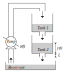
\includegraphics[width=0.48\textwidth]{Chapter6_CaseStudies/TanksSchematic.pdf}
\caption{Diagram of cascaded tanks benchmark system with typical water flow}
\label{fig:System_Tanks}
\end{figure}

Ignoring saturation, the system is weakly nonlinear based on the flow equations through the valves in each tank, which can be derived from Bernoulli's principle. The system also contains a hard nonlinearity in the form of water level saturation. Once the maximum level of either tank is reached, an overflow occurs. Furthermore, saturation in the top tank introduces input-dependent process noise, since some of the overflowing water can fall into the lower tank and affect the output. 

\subsection{Measurement process}

Two sets of data have been recorded for the benchmark: an estimation set and a validation set. For both datasets, the voltage input to the tank system is excited using one period of a multisine which excites frequencies from 0 to 0.0144 Hz. Using a sampling period of $T_s=4$s, this gives input vectors of length $N=1024$. The corresponding output measurements are obtained from the capacitive level sensor of the lower tank, which may introduce measurement noise. The system is not in steady state during the measurement window, and the initial states of the system are unknown but approximately equal for both datasets. The recorded signals are plotted in Figure \ref{fig:datasets_tanks} in the time domain (top) and frequency domain (bottom). While the hard saturation nonlinearity is clearly visible in the time domain output signals, there is also evidence of nonlinearity in the frequency domain, where some output power exists at unexcited frequencies.

\begin{figure}[h]
\centering
\includegraphics[width=1.05\textwidth]{Chapter6_CaseStudies/Datasets_tanks.pdf}
\caption{Estimation (blue) and validation (red) datasets for the cascaded tanks in the time (top) and frequency (bottom) domain}
\label{fig:datasets_tanks}
\end{figure}

\subsection{Problem statement}

To maintain consistency with the estimates obtained in \cite{Birpoutsoukis2017b}, the identification problem is considered exactly as stated in the benchmark document \cite{Schoukens2016c}. The required outcome is to identify a model of the system using the estimation dataset, and report the accuracy of the estimated model in predicting the output of the \emph{entire} $1024$-sample validation dataset using the following metric, 
\begin{equation}
e_{RMSt} = \sqrt{\frac{1}{N_v} \sum_{t=1}^{N_v} (y_{mod}(t) - y_v(t) )^2},
\label{eq:e_RMSt}
\end{equation}
where $N_v = 1024$ is the length of $y_v$, the validation output, and $y_{mod}$ is the modeled output for the same validation input. Note that prediction of the entire output vector requires estimation of the unknown initial states, since the start of the record will be affected by inputs applied prior to the measurement window. 

\subsection{Estimating unknown initial states}

In the nonparametric Volterra series context, the initial states problem becomes an issue of `past inputs', since Volterra kernel outputs are functions of lagged inputs only. Hence, in order to estimate/validate using the entire output vector, $\{y(t)\}_{t=1}^{1024}$, we require knowledge of $u(t)$ for $n<t<0$ and some reasonable memory length $n$. Of course, no knowledge of these past inputs can be gained from the provided datasets, so two strategies are discussed in this section in order to continue estimating/validating with the complete output vector. Both strategies are applied to the benchmark data in Section \ref{sec:Results_tanks}.

\subsubsection{Bayesian transient estimation}
\label{sec:BayesTrans_tanks}

For consistency, one approach we consider is the method used in \cite{Birpoutsoukis2017b}, whose results will be the subject of comparison for this benchmark. In the paper, which relies on previous results established in \cite{Csurcsia2015}, the input is assumed to be periodic, i.e. $u(t-N) = u(t) \; \forall t$, where $N=1024$ for the cascaded tanks. However, since the system is not in steady state, this assumption is clearly in error, and we expect to see a `transient' function which describes the difference between the measured output and the ideal steady-state output. This difference will be denoted $\theta_{tr}$, which has length $n_{tr}<N$.

In this case, the regression structure for basis function kernels in (\ref{eq:RegressionStructure_OBFseries}) can be updated to include the transient,
\begin{equation}
Y = \Phi_f^T \alpha + \Phi_{\delta} \theta_{tr} + E,
\end{equation}
where the $Y$ vector now contains all $N$ samples of $y(t)$, $\Phi_f$ contains measured \emph{and} unmeasured input values, and $\Phi_{\delta}$ is a $N \times n_{tr}$ rectangular identity. Staying within the Bayesian framework, a Gaussian assumption is placed on $\theta_{tr}$, such that the regularization problem can be augmented as follows,
\begin{align}
&\alpha' = [\alpha^T \; \; \theta_{tr}^T]^T, \; \; \Phi' = [\Phi_f^T \; \; \Phi_{\delta}], \nonumber \\
&\hat{\alpha}'_{ReLS} = \text{arg } \underset{\alpha'}{\text{min}} \|Y - \Phi' \alpha' \|^2_2 + \sigma^2 \alpha'^T [P']^{-1} \alpha',
\end{align}
where $P'$ is an augmented prior covariance matrix given by
$$P' = \begin{bmatrix}
       P &  \mathbf{0} \\
        \mathbf{0}  & P_{tr}
     \end{bmatrix},$$
and $P_{tr}$ is the covariance of $\theta_{tr}$, which is chosen to have the linear DC structure\footnote{While the DC structure imposes smoothness on the estimated transient, we will see in Chapter \ref{chap:9} that Volterra system transients may also include a non-smooth component. Here, the non-smooth component will be captured by $E$.} given in (\ref{eq:DCstructure}). The prior covariance, $P$, for the original parameter vector, $\alpha$, is also chosen to be DC-based and is constructed as in previous chapters using (\ref{KernelPenalty}), (\ref{DCext}), and (\ref{FinalPenalty}).

The hyperparameter set, $\eta$ (which now includes hyperparameters for $P_{tr}$) is still tuned with EM using Algorithm \ref{alg:BFopt}, however some minor modifications are made to include the augmented transient components. The $P_{tr}$ hyperparameters are then re-used in the validation dataset, to re-estimate and remove the transient function from the output.

\subsubsection{Constant past input assumption}
\label{sec:ConstInput_tanks}

An alternate solution to the unknown initial states problem can be formulated, which adds less complexity to the EM optimization and requires no re-estimation on the validation data. In this approach, we restrict the unmeasured input, $\{u(t)\}_{t=-\infty}^{-1}$ to the class of constant sequences, i.e.
$$u(t) = c \; \; \forall t<0; \; c \in \mathbb{R}^+.$$ 
The constant, $c$, is tuned during the optimization in Algorithm \ref{alg:BFopt} such that the following condition is satisfied in each iteration: 
$$y_P^{(k)}(0) = y(0),$$ 
where $y_P^{(k)}(0)$ is the output value predicted using $\hat{\alpha}^{(k)}$ and past inputs $u(t)=c$ for $t<0$ in the regressor, $\Phi_f$.  

\subsection{Identification results}
\label{sec:Results_tanks}

The regularized estimation method from Chapter \ref{chap:5} (ReLBF) is applied for several orders of the model structure in (\ref{OBFvolterra}) expanded using Laguerre basis functions:
\begin{itemize}
\item A linear LBF expansion, i.e. excluding $\alpha_0$ and setting $M=1$
\item A 2nd order Volterra-Laguerre series (M=2)
\item A 3rd order Volterra-Laguerre series (M=3)
\end{itemize}

The truncation lengths at each order are chosen as $\mathcal{B}_1 = 15$, $\mathcal{B}_2 = 10$ and $\mathcal{B}_3$ = 8, having been obtained through a typical iterative identification process. For the Bayesian transient removal method \cite{Birpoutsoukis2017b}, the length of the transient is $n_{tr} = 100$.

Hyperparameter optimization is achieved using the MATLAB $\text{\tt{GlobalSearch}}$ and $\text{\tt{fmincon}}$ functions to perform all non-convex minimizations in Algorithm \ref{alg:BFopt}. Computation times for the estimation are measured on an Intel Xeon 3.50 GHz processor.

The two methods for dealing with unknown initial states are denoted `Bayesian transient' for the first method in Section \ref{sec:BayesTrans_tanks} and `Constant input' for the second method.

\subsubsection{Estimation and validation}

Modeling the system first with a linear LBF expansion, a reasonable result is achieved, but the shortcomings of a linear model are clear. The estimated LBF coefficients are plotted in Figure \ref{fig:LinearTankEst}, along with the corresponding time-domain impulse response. The choice of $\mathcal{B}_1=15$ is supported by the estimate, and the decay time of the impulse response suggests that $n_{tr}=100$ is a reasonable choice, since the transient function typically decays at the same rate as the system response, at least for linear systems \cite{Lataire2016}.

\begin{figure}[h]
\centering
\includegraphics[width=0.9\textwidth]{Chapter6_CaseStudies/LinearLBFs.pdf}
\caption{Linear model for the cascaded tanks: estimated LBF coefficients (left) and equivalent time domain FIR (right)}
\label{fig:LinearTankEst}
\end{figure}

\begin{figure}[h]
\centering
\includegraphics[width=0.9\textwidth]{Chapter6_CaseStudies/LinearValidation.pdf}
\caption{Linear model for the cascaded tanks: true (black) and modeled (red) validation outputs using both transient removal methods}
\label{fig:LinearTankVal}
\end{figure}

The true and modeled validation outputs for the linear estimate are given in Figure \ref{fig:LinearTankVal}, where we see that the modeled output is quite poor in the first half of the record. The Bayesian transient approach is also seen to produce a better result than the constant input assumption, although it relies on some estimation using the validation data. Overall, there is clearly room for improvement, which can likely be achieved by estimating higher order terms of the Volterra-Laguerre series.

Estimating a second order Volterra-Laguerre model, the validation performance is significantly improved. The constant kernel is estimated as $\hat{\alpha}_0 = -4.55$, and the first and second order basis function kernels are plotted in Figure \ref{fig:2ndOrderTankEst}. The true and modeled validation outputs are given in Figure \ref{fig:2ndOrderTankVal}, where it can be observed that the output predicted by the model is visibly more accurate than in the linear case. Furthermore, the Bayesian transient and constant input methods both obtain a good prediction of the initial 100 output samples. 

\begin{figure}[h]
\centering
\includegraphics[width=0.9\textwidth]{Chapter6_CaseStudies/Kernels2ndOrder_CT_Coloured.pdf}
\caption{Volterra model (M=2) for the cascaded tanks: estimated 1st order (left) and 2nd order (right) LBF kernels}
\label{fig:2ndOrderTankEst}
\end{figure}

\begin{figure}[h]
\centering
\includegraphics[width=0.9\textwidth]{Chapter6_CaseStudies/2ndOrderValidation.pdf}
\caption{Volterra model (M=2) for the cascaded tanks: true (black) and modeled (red) validation outputs using both transient removal methods}
\label{fig:2ndOrderTankVal}
\end{figure}

The third order Volterra-Laguerre model has aso been estimated, however the improvement in validation performance is negligible with respect to the second order model. The error metrics and computation times are still reported.

The RMS error in the validation is computed for each model and method using (\ref{eq:e_RMSt}), and these errors are compared, in Table \ref{tab:eRMS_tanks}, with the time domain results reported in \cite{Birpoutsoukis2017b}. The results show very similar validation performance between the time domain and LBF approach. The constant input method of transient removal is seen to provide essentially the same accuracy as the Bayesian method (with the exception of the linear case), despite its more simple nature. 

\renewcommand{\arraystretch}{1.3}
\begin{table}[h]
\centering
\caption{Comparison of validation errors between methods}
\label{tab:eRMS_tanks}
\begin{tabular}{|l||r|r|r|}
\hline
                & \multicolumn{3}{c|}{\textbf{$\mathbf{e_{RMSt}}$ (from (\ref{eq:e_RMSt}))}} \\ \cline{2-4} 
\textbf{Model} & Birpoutsoukis           & ReLBF            & ReLBF                \\ 
		&  et. al. (2017) \cite{Birpoutsoukis2017b}          & (Bayesian)           & (Constant)                \\ \hline 
Linear         & 0.84              & 0.85             & 0.91                            \\ \hline
Volterra (M=2)         & 0.55               & 0.56             & 0.57                             \\ \hline
Volterra (M=3)           & 0.54              & 0.56             & 0.56                             \\ \hline
\end{tabular}
\end{table}

While the validation performance of the time domain and basis function Volterra models is extremely similar for the cascaded tanks benchmark, significant advantages of the basis function formulation can be seen when comparing the numbers of unique parameters required, and the computation time required for model estimation. In Table \ref{tab:Params+Times_tanks}, the total parameter numbers and computation times are reported for the LBF method, alongside the corresponding figures for the time domain approach as reported in \cite{Birpoutsoukis2017c}. It is clear that a LBF formulation of the regularized problem produces far more compact Volterra models, with an order of magnitude difference in the parameter numbers. As a direct consequence, the difference in computation time is even greater, where the Volterra-Laguerre estimates are computed two or three orders of magnitude faster.

\renewcommand{\arraystretch}{1.3}
\begin{table}[h]
\centering
\caption{Comparison of computation time and parameter numbers between methods}
\label{tab:Params+Times_tanks}
\begin{tabular}{|l||c|c||c|c|}
\hline
                & \multicolumn{2}{c||}{\textbf{Parameters}} & \multicolumn{2}{c|}{\textbf{Comp. Time (mins)}}  \\ \cline{2-5} 
\textbf{Model} & Time domain         & ReLBF            &Time domain           & ReLBF                \\ \hline
Linear                   & 92                     & 15    &   3          &  0.1 \\ \hline
Volterra (M=2)                 & 721      &  71        & 210             &  0.6                \\ \hline
Volterra (M=3)                     & 860      & 191      & 390             &  2                 \\ \hline
\end{tabular}
\end{table}

%---------------------------------------------------------------------------------------------------------------------------------------------------------------------------------------------------------------------------------------

\section{Coupled electric drives}

The coupled electric drives is a benchmark system inspired by an example which appeared in \cite{Wellstead1979}. The original example was designed to represent machines which transfer a belt of material from one spool to another using two electric drives and a pulley. In the benchmark problem, a data set of only 500 samples is provided for estimation purposes. The system has previously been modeled using block-oriented models, where the structure is derived from knowledge of the relevant physical interactions \cite{Wigren2017}. As was done for the cascaded tanks benchmark, here the identification problem will be approached from a position of no prior knowledge, to highlight the versatility of Volterra series modeling even when using an extremely short estimation dataset. The comparison for the drives system will be between regularized basis function estimates (using ReLBF) and estimates obtained using several other popular nonlinear model classes. 

\subsection{System description}
\label{sec:CED_description}

The benchmark system is configured as shown in Figure \ref{fig:CoupledDrivesSchematic}, where the input is simultaneously applied to two motors driving a flexible belt, which in turn rotates a pulley being held by a spring. The angular speed of the pulley is measured by a pulse transducer, whose measurement is sent through an analogue low-pass and anti-aliasing filter to produce the final speed output which can be used for control purposes.  

\begin{figure}[h]
\centering
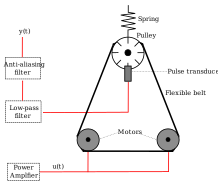
\includegraphics[width=0.75\textwidth]{Chapter6_CaseStudies/DrivesSchematic.pdf}
\caption{Schematic of the coupled electric drives benchmark system} \label{fig:CoupledDrivesSchematic}
\end{figure}

The spring and flexible belt add lightly damped dynamic modes to the system, and there will also be time constants associated with the motors, however these are all linear effects. The modeling complication is brought about by the pulse transducer, which is insensitive to the \emph{direction} of rotation of the pulley, since it simply counts pulses to approximate angular velocity. As the motors can be driven in either direction, the transducer can be considered as having an `absolute value' nonlinearity, such that the total system is well approximated by a Wiener-Hammerstein block structure, as depicted in Figure \ref{fig:WienerHamm_CED}. 

\begin{figure}[h]
\centering
\includegraphics[scale = 1]{Chapter6_CaseStudies/WienerHammCED.pdf}
\caption{Wiener-Hammerstein block structure for the coupled electric drives} \label{fig:WienerHamm_CED}
\end{figure}

\subsection{Measurement process}

While some physical modeling insights can be obtained by analyzing the system set-up, it is the experimental input-output data which will be used to identify and assess candidate models. An estimation and a validation dataset have been recorded, both containing 500 input-output samples recorded at 50 Hz. The inputs are constructed from a Pseudo-Random Binary Sequence (PRBS) which is multiplied by a noise sequence with uniform distribution. The input and output signals for each set are shown in Figure \ref{fig:EstimationData_CED}. The validation input is seen to be the estimation input shifted by an offset of +0.5V, and the absolute value nonlinearity is clearly visible in the output signals.

\begin{figure}[h]
\centering
\includegraphics[width=0.95\textwidth]{Chapter6_CaseStudies/Datasets_drives.pdf}
\caption{Input (top) and output (bottom) signals for the coupled electric drives estimation (blue) and validation (red) datasets} \label{fig:EstimationData_CED}
\end{figure}

\subsection{Problem statement}

The identification problem for the coupled electric drives is to estimate a nonlinear model using the estimation data, and use this model to predict the output for the validation dataset. Unlike the cascaded tanks benchmark, the issue of estimating initial states will not be considered. Instead, the model predicted output begins at the 60\textsuperscript{th} sample, when enough measured input information is available.

The performance of each nonlinear model on the validation data is assessed numerically, using a normalized root mean square error (NRMSE) metric defined by 
\begin{equation}
\text{NRMSE} = \frac{||Y_{val}-Y_{mod}||_2}{||Y_{val} - \text{mean}(Y_{val}) ||_2},
\label{eqn:NRMSE_CED}
\end{equation}
where $Y_{val}$ is the true validation output vector and $Y_{mod}$ is the model-predicted output vector.

\subsection{Identification results}
\label{sec:Results_CED}

LBF-expanded Volterra kernels are estimated for the benchmark system using the ReLBF method proposed in Chapter \ref{chap:5}. Due to the limited number of estimation samples available, the order of the Volterra series is fixed at $M=2$, and using no prior knowledge of the system, the number of basis functions for each order is chosen to be $\mathcal{B}_1=\mathcal{B}_2=20$, such that the total number of unique parameters requiring estimation (231) is roughly half the number of data samples available. All non-convex optimization problems in Algorithm \ref{alg:BFopt} are solved using the MATLAB $\text{\tt{GlobalSearch}}$ and $\text{\tt{fmincon}}$ functions to locate a global minimum.

\begin{figure}[!b]
\centering
\includegraphics[width=\textwidth]{Chapter6_CaseStudies/Kernels2ndOrder_CED_Coloured}
\caption{Estimated 2\textsuperscript{nd} order LBF kernel (left) and its time domain equivalent (right) for the coupled electric drives} \label{fig:Kernel2_CED}
\end{figure}

The first order kernel, $\hat{\alpha}_1$, is estimated to be negligible. This is to be expected, since the absolute value nonlinearity is an \emph{even} function and as such generates only even order Volterra kernels in the series expansion. The second order LBF kernel estimate, $\hat{\alpha}_2$, is shown in Figure \ref{fig:Kernel2_CED} as well as its time domain equivalent, $\hat{h}_2$. The zeroth order kernel is estimated as $\hat{\alpha}_0 = 0.102$.

Applying the validation input to the estimated Volterra-Laguerre model produces the output prediction shown in Figure \ref{fig:ValidationLBFVK_CED}, which is plotted with the given validation output. Despite using only 500 samples for estimation, the regularized basis function approach provides a very accurate model which is suitable for prediction or control purposes. 

\begin{figure}[h]
\centering
\includegraphics[width=\textwidth]{Chapter6_CaseStudies/ValidationLBFVK_CED.pdf}
\caption{True and model-predicted validation outputs for the Volterra-Laguerre model applied to the coupled electric drives benchmark} \label{fig:ValidationLBFVK_CED}
\end{figure}

\subsubsection{Comparison with Alternate Methods }

In order to provide some context when assessing the performance of the proposed method, several alternate model classes and methods are also applied to the coupled electric drives benchmark. The other models considered are:
\begin{enumerate}
\item Linear state space 
\item Linear transfer function 
\item Nonlinear ARX (NARX) 
\item Wiener block structure
\end{enumerate}

For each model class, the estimation dataset is used to estimate a model using the appropriate method provided by MATLAB's System Identification toolbox. As in the proposed ReLBF method, no prior knowledge is used in the estimation, and the model orders for each case are chosen based on a cross-validation approach. High order polynomials are used for nonlinear function estimates. Note that Wiener-Hammerstein models cannot be estimated using the toolbox, however this case has already been treated in~\cite{Wigren2017}.

The predicted validation output from each model is plotted in Figure \ref{fig:ValidationToolbox_CED}, along with the true experimental output (in black). It is clear that for such a short estimation dataset, and without the use of prior knowledge, none of the estimated models provide accurate predictions over the entire validation set for the coupled electric drives system. 

\begin{figure}[h]
\centering
\includegraphics[width=\textwidth]{Chapter6_CaseStudies/ToolboxValidations_CED.pdf}
\caption{True and model-predicted validation outputs for toolbox methods in MATLAB applied to the coupled electric drives benchmark} \label{fig:ValidationToolbox_CED}
\end{figure}

The NRMSE error metric (\ref{eqn:NRMSE_CED}) for each toolbox method is compared in Table \ref{tab:NRMSE_CED} against the method proposed in this thesis (ReLBF), highlighting the superior performance of the regularized nonparametric approach. From the four toolbox models, the Wiener structure produces the next best validation results, which can be attributed to the Wiener-Hammerstein nature of the true system (see Figure \ref{fig:WienerHamm_CED}), where the final linear filter block contains dynamics which could be considered negligible. This is further supported by the fact that similar prediction performance was achieved using a Wiener-Hammerstein model in \cite{Wigren2017}.

\begin{table}[h]
\centering
\caption{NRMSE in validation for proposed and toolbox methods}
\begin{tabular}{|c||c|c|c|c|c|}
\hline
\textbf{Model} & State Space & Transfer Func. & NARX & Wiener &\emph{ReLBF} \\
\hline
\textbf{NRMSE} & 0.598 & 0.543 & 0.554 & 0.361 & 0.189 \\
\hline
\end{tabular}
\label{tab:NRMSE_CED}
\end{table}

\section{Conclusion}

The Volterra series has historically been regarded as an impractical tool for data-driven modeling. The benchmark examples in this chapter, however, have shown that by using a more compact basis function formulation, and efficiently regularizing the estimation to impose known properties of smoothness and decay, the Volterra series \emph{can} be a broad and powerful tool for nonlinear system identification. 

The cascaded tanks benchmark revealed that a regularized basis function method can be adapted to deal with unknown initial states in a system. The resulting 2\textsuperscript{nd} and 3\textsuperscript{rd} order series estimates gave reasonably accurate prediction performance, despite the short data record used for estimation. This performance was compared against the time domain estimation method in \cite{Birpoutsoukis2017b}, showing equivalent validation metrics but a stark decrease in parameter numbers and computation times for the proposed basis function approach. 

The coupled electric drives benchmark provided further evidence for the proposed method. Despite having an even shorter estimation dataset of 500 samples, and without incorporating prior knowledge of the drives system into the modeling process, the estimated Volterra-Laguerre kernels provided accurate predictions in the validation step. Furthermore, the proposed method significantly outperformed linear and nonlinear models provided by the established System Identification toolbox in MATLAB in terms of the considered error metric.